\documentclass[tikz,border=4pt]{standalone}
\usepackage{amsmath,amssymb,bm}
\usetikzlibrary{positioning,arrows.meta,fit,backgrounds,calc}
\begin{document}
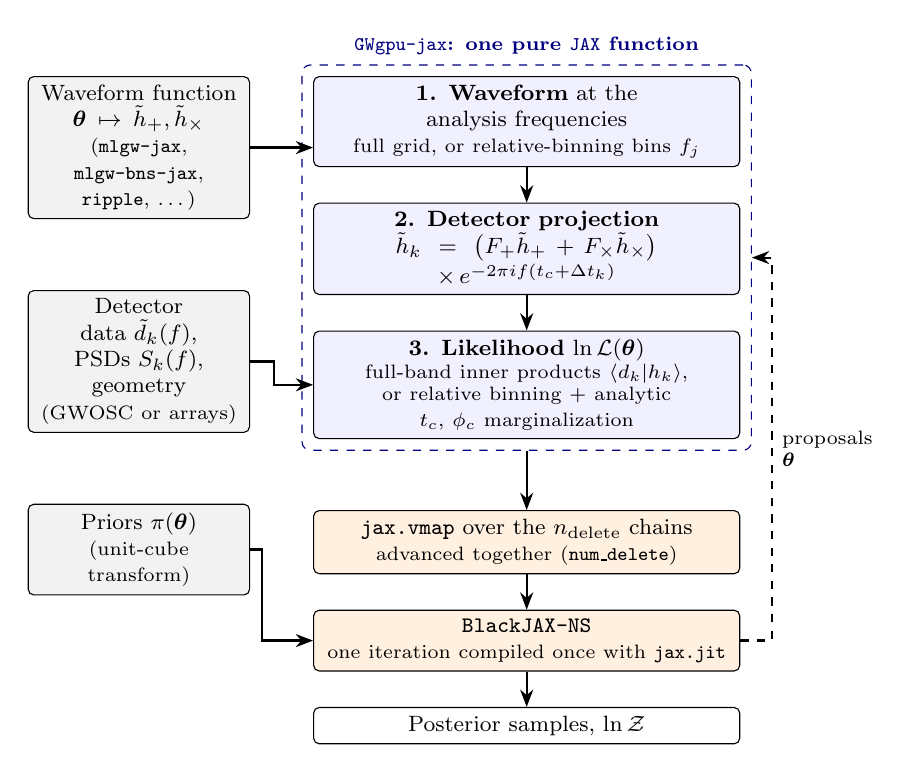
\begin{tikzpicture}[
    font=\footnotesize,
    node distance=4.5mm and 4mm,
    box/.style={draw, rounded corners=2pt, align=center, inner sep=3pt, text width=#1},
    box/.default=37mm,
    inp/.style={box=26mm, fill=gray!10},
    core/.style={box=52mm, fill=blue!6},
    smp/.style={box=52mm, fill=orange!12},
    arr/.style={-{Stealth[length=2.2mm]}, thick},
]
% ---------------- inputs ----------------
\node[inp] (wf) {Waveform function\\ $\bm\theta \mapsto \tilde h_{+}, \tilde h_{\times}$\\ \scriptsize (\texttt{mlgw-jax}, \texttt{mlgw-bns-jax}, \texttt{ripple}, \ldots)};
\node[inp, below=9mm of wf] (data) {Detector data $\tilde d_k(f)$,\\ PSDs $S_k(f)$, geometry\\ \scriptsize (GWOSC or arrays)};
\node[inp, below=9mm of data] (prior) {Priors $\pi(\bm\theta)$\\ \scriptsize (unit-cube transform)};

% ---------------- likelihood core ----------------
\node[core, right=8mm of wf.north east, anchor=north west] (gen) {\textbf{1. Waveform} at the analysis frequencies\\ \scriptsize full grid, or relative-binning bins $f_j$};
\node[core, below=of gen] (proj) {\textbf{2. Detector projection}\\ $\tilde h_k = \bigl(F_{+}\tilde h_{+} + F_{\times}\tilde h_{\times}\bigr)$\\ $\times\, e^{-2\pi i f (t_c+\Delta t_k)}$};
\node[core, below=of proj] (like) {\textbf{3. Likelihood} $\ln\mathcal{L}(\bm\theta)$\\ \scriptsize full-band inner products $\langle d_k|h_k\rangle$,\\ \scriptsize or relative binning $+$ analytic\\ \scriptsize $t_c$, $\phi_c$ marginalization};
\begin{scope}[on background layer]
\node[draw=blue!50!black, dashed, rounded corners=3pt, inner sep=4pt, fit=(gen)(proj)(like),
      label={[font=\scriptsize\bfseries, text=blue!50!black]above:\texttt{GWgpu-jax}: one pure \texttt{JAX} function}] (gw) {};
\end{scope}

% ---------------- sampler ----------------
\node[smp, below=9mm of like] (vmap) {\texttt{jax.vmap} over the $n_{\rm delete}$ chains\\ \scriptsize advanced together (\texttt{num\_delete})};
\node[smp, below=of vmap] (ns) {\textbf{\texttt{BlackJAX-NS}}\\ \scriptsize one iteration compiled once with \texttt{jax.jit}};
\node[box=52mm, below=of ns] (out) {Posterior samples, $\ln\mathcal{Z}$};

% ---------------- arrows ----------------
\draw[arr] (data.east) -- ++(3mm,0) |- (like.west);
\draw[arr] (wf.east) -- (wf.east -| gen.west);
\draw[arr] (prior.east) -- ++(1.5mm,0) |- (ns.west);
\draw[arr] (gen) -- (proj);
\draw[arr] (proj) -- (like);
\draw[arr] (gw.south) -- (vmap);
\draw[arr] (vmap) -- (ns);
\draw[arr] (ns) -- (out);
\draw[arr, dashed] (ns.east) -- ++(4mm,0) |- node[pos=0.25, right, font=\scriptsize, align=left] {proposals\\ $\bm\theta$} (gw.east);
\end{tikzpicture}
\end{document}
